% ---------------------------------
% Formato IEEE (conferencia) - clase IEEEtran
% ---------------------------------
\documentclass[conference]{IEEEtran}
\IEEEoverridecommandlockouts

% ------------------------ PAQUETES
\usepackage[utf8]{inputenc}
\usepackage[T1]{fontenc}
\usepackage[spanish]{babel}
\usepackage{cite}
\usepackage{amsmath,amssymb,amsfonts}
\usepackage{bbm}
\usepackage{mathrsfs}
\usepackage{graphicx}
\usepackage{array}
\usepackage{textcomp}
\usepackage{xcolor}
\usepackage{url}
\usepackage[section]{placeins}
\urlstyle{same}
\def\UrlBreaks{\do\/\do-\do_\do.\do=\do?\do\&} % Permite cortar URLs largas
\def\BibTeX{{\rm B\kern-.05em{\sc i\kern-.025em b}\kern-.08em
    T\kern-.1667em\lower.7ex\hbox{E}\kern-.125emX}}

% -------------------- DEFINICIONES
\def\R{\mathbbm{R}} %Conjunto de los números reales
\def\C{\mathbbm{C}} %Conjunto de los números complejos
\def\Cf{\mathcal{C}}%Conjunto de las funciones continuas
\def\dt{\,\text{d}t}
\def\ds{\,\text{d}s}
\def\dy{\,\text{d}y}
\def\du{\,\text{d}u}
\def\L{\mathscr{L}} %Transformada de Laplace
\newcommand{\crc}{\textcolonmonetary} % Símbolo ₡
% ---------------------------------
\definecolor{gris}{cmyk}{0,0,0,0.1}
\definecolor{greenJu}{rgb}{0.0, 0.5, 0.0}
\definecolor{miAzul}{RGB}{0, 0, 255}   % Azul puro
\definecolor{miRojo}{RGB}{255, 0, 0}   % Rojo puro
\definecolor{miVerde}{RGB}{21, 45, 15}  % Verde puro

% Salto de fila entre autores (IEEEtran centra cada fila)
\makeatletter
\newcommand{\linebreakand}{%
  \end{@IEEEauthorhalign}
  \hfill\mbox{}\par
  \mbox{}\hfill\begin{@IEEEauthorhalign}
}
\makeatother




\begin{document}

\renewcommand{\IEEEkeywordsname}{Palabras clave}
% ---------------------------------
% TITULO Y AUTORES
% ---------------------------------
\title{An\'alisis exploratorio y predictivo del comportamiento comercial de las empresas distribuidoras de energ\'ia el\'ectrica en Costa Rica entre enero de 2025 y agosto de 2026 mediante t\'ecnicas de an\'alisis de datos utilizando Python}


    
\author{
\IEEEauthorblockN{Ana Luc\'ia Salazar Chac\'on}
\IEEEauthorblockA{Escuela de Inform\'atica\\
Universidad Nacional de Costa Rica\\
Heredia, Costa Rica\\
ana.salazar.chacon@est.una.ac.cr}
\and
\IEEEauthorblockN{Nicolas Z\'arate Hern\'andez}
\IEEEauthorblockA{Escuela de Inform\'atica\\
Universidad Nacional de Costa Rica\\
Heredia, Costa Rica\\
nicolas.zarate.hernandez@est.una.ac.cr}
\and
\IEEEauthorblockN{Gerson Jafet Madrigal Cubillo}
\IEEEauthorblockA{Escuela de Inform\'atica\\
Universidad Nacional de Costa Rica\\
Heredia, Costa Rica\\
gerson.madrigal.cubillo@est.una.ac.cr}
\linebreakand
\IEEEauthorblockN{Sandy Marchena Blanco}
\IEEEauthorblockA{Escuela de Inform\'atica\\
Universidad Nacional de Costa Rica\\
Heredia, Costa Rica\\
sandy.marchena.blanco@est.una.ac.cr}
}



\maketitle

\begin{abstract}
Este trabajo analiza y pronostica a corto plazo los precios medios de la electricidad de los cuatro principales operadores p\'ublicos de distribuci\'on de Costa Rica entre enero de 2025 y agosto de 2026, a partir de los datos abiertos del ente regulador. Con un flujo reproducible en Python se calcul\'o el precio medio ponderado mensual con y sin el Costo Variable de Generaci\'on (CVG), se ajustaron modelos de regresi\'on lineal, uno simple y otro con una variable indicadora, y se evalu\'o su capacidad predictiva frente a un pron\'ostico ingenuo. En 2026 el precio baj\'o hasta un 13,9\,\% respecto de 2025, sin que disminuyeran las ventas. Los precios no siguen una tendencia, sino un cambio de nivel en febrero de 2026, explicado porque el CVG pas\'o de recargo a descuento y no por una baja de la tarifa base. Ning\'un modelo super\'o al pron\'ostico ingenuo, con errores menores al 2\,\%.
\end{abstract}

\begin{IEEEkeywords}
precios medios, energ\'ia el\'ectrica, ARESEP, Costo Variable de Generaci\'on, regresi\'on lineal, an\'alisis de datos, Python
\end{IEEEkeywords}



% ---------------------------------
\section{Introducci\'on}
\label{sec:intro}

En Costa Rica, el precio de la electricidad no lo fija el mercado, sino la Autoridad Reguladora de los Servicios P\'ublicos (ARESEP), que lo establece mediante resoluciones administrativas bajo el principio de servicio al costo~\cite{r3}. A las tarifas base se suma el Costo Variable de Generaci\'on (CVG), un ajuste extraordinario que traslada a las tarifas las variaciones del costo de generaci\'on, en particular de la generaci\'on t\'ermica, muy sensible a la hidrolog\'ia~\cite{r2}. Tras el evento de El Ni\~no de 2023 y 2024, este componente represent\'o un recargo considerable durante 2025, y su evoluci\'on posterior incide directamente en el precio que pagan los usuarios y en los ingresos de las empresas distribuidoras.

La ARESEP publica en su portal de datos abiertos, con detalle mensual, los ingresos, las ventas y los precios medios de cada empresa distribuidora y tipo de tarifa, con y sin el CVG~\cite{r6}. Estos datos permiten observar c\'omo se traducen las decisiones regulatorias en el precio efectivo de la energ\'ia, pero su volumen y desagregaci\'on exigen un procesamiento sistem\'atico. Los estudios nacionales sobre tarifas el\'ectricas se han centrado en el an\'alisis jur\'idico y de pol\'itica p\'ublica~\cite{r9}, y no se identific\'o un an\'alisis cuantitativo reciente de los precios medios por operador.

El objetivo de este trabajo es describir y modelar el comportamiento del precio medio de la electricidad de los cuatro principales operadores de distribuci\'on: el Instituto Costarricense de Electricidad (ICE), la Compa\~n\'ia Nacional de Fuerza y Luz (CNFL), la Empresa de Servicios P\'ublicos de Heredia (ESPH) y la Junta Administrativa del Servicio El\'ectrico de Cartago (JASEC), entre enero de 2025 y agosto de 2026, y determinar en qu\'e medida sus cambios responden a la tarifa base o al CVG. Para ello se desarroll\'o en Python un flujo reproducible que obtiene los datos desde el servicio web de la ARESEP, los depura, los explora, ajusta dos modelos de regresi\'on lineal, uno simple y otro con una variable indicadora del cambio de nivel de 2026, y eval\'ua su capacidad predictiva a corto plazo.

El art\'iculo se organiza de la siguiente manera. La Secci\'on~\ref{sec:marco} presenta el marco te\'orico y la Secci\'on~\ref{sec:metodologia}, la metodolog\'ia de obtenci\'on y limpieza de los datos. La Secci\'on~\ref{sec:eda} expone el an\'alisis exploratorio, y la Secci\'on~\ref{sec:regresion}, los modelos de regresi\'on y la evaluaci\'on predictiva. Por \'ultimo, la Secci\'on~\ref{sec:discusion} discute los resultados y la Secci\'on~\ref{sec:conclusiones} presenta las conclusiones.


% ---------------------------------
\section{Marco te\'orico}
\label{sec:marco}
El estudio del comportamiento comercial de las empresas distribuidoras de electricidad exige articular dos cuerpos de conocimiento: la regulaci\'on econ\'omica del servicio el\'ectrico costarricense, que determina c\'omo se forman los precios, y las t\'ecnicas de an\'alisis de datos que permiten describir y proyectar ese comportamiento. El presente marco recorre ambos y responde a una pregunta articuladora: por qu\'e resulta relevante analizar los precios medios y los ingresos de la electricidad, y por qu\'e Python constituye una herramienta adecuada para hacerlo.

% ---------------------------------
\subsection{Sector el\'ectrico costarricense}
\label{sec:electricidadCR}
Costa Rica conserv\'o un modelo de servicio el\'ectrico p\'ublico integrado, de propiedad estatal, municipal y cooperativa, en el que la competencia por el mercado fue sustituida por una regulaci\'on econ\'omica de car\'acter administrativo. La etapa de distribuci\'on, foco de esta investigaci\'on, es donde se materializan los ingresos comerciales de las empresas y est\'a a cargo de ocho operadores con zonas de concesi\'on exclusivas: el Instituto Costarricense de Electricidad (ICE), la Compa\~n\'ia Nacional de Fuerza y Luz (CNFL), la Empresa de Servicios P\'ublicos de Heredia (ESPH), la Junta Administrativa del Servicio El\'ectrico de Cartago (JASEC) y las cooperativas Coopelesca, Coopeguanacaste, Coopesantos y Coopealfaroruiz~\cite{r1}. Son unidades muy heterog\'eneas en escala y densidad de abonados, por lo que su comparaci\'on exige normalizar previamente las variables y delimitar cu\'ales de ellas se incluyen en el estudio, como se detalla en la Secci\'on~\ref{sec:delimitacion}.

La matriz de generaci\'on es predominantemente hidroel\'ectrica, de modo que el costo de abastecimiento del sistema depende de la hidrolog\'ia. Durante el evento de El Ni\~no de 2023 y 2024, la generaci\'on t\'ermica, seg\'un los datos abiertos del Grupo ICE~\cite{r2}, pas\'o de aproximadamente un 0,7\,\% a un 7,5\,\% del total de la generaci\'on el\'ectrica nacional, y ese encarecimiento se traslada a las tarifas y, por esa v\'ia, a los ingresos de las distribuidoras.

% ---------------------------------
\subsection{Delimitaci\'on del estudio}
\label{sec:delimitacion}

Del conjunto de ocho operadores descrito, esta investigaci\'on delimita su alcance a los cuatro operadores p\'ublicos de mayor cobertura y volumen de abonados: el ICE, la CNFL, la ESPH y JASEC. El criterio de selecci\'on utilizado fue la cobertura geogr\'afica y el tama\~no de la cartera de abonados: estos cuatro operadores concentran zonas de concesi\'on de alcance nacional o metropolitano (el ICE opera en gran parte del territorio nacional, la CNFL en la Gran \'Area Metropolitana, la ESPH en el cant\'on de Heredia y JASEC en el cant\'on de Cartago~\cite{r1}), mientras que las cooperativas de electrificaci\'on rural (Coopelesca, Coopeguanacaste, Coopesantos y Coopealfaroruiz) atienden zonas de concesi\'on rurales, de menor densidad de abonados y bajo un modelo de gesti\'on cooperativo distinto al de estos operadores. Por esa heterogeneidad de escala y de modelo de gesti\'on, una comparaci\'on directa entre ambos grupos no resultar\'ia metodol\'ogicamente adecuada, por lo que las cooperativas quedan fuera del alcance de este estudio.

En cuanto al periodo de an\'alisis, se utilizar\'an los datos mensuales de precios medios e ingresos publicados por la ARESEP correspondientes al a\~no 2025 completo (enero a diciembre) y al periodo de enero a agosto de 2026. Dado que el consumo el\'ectrico presenta estacionalidad, las comparaciones entre operadores se realizar\'an \'unicamente entre periodos equivalentes de ambos a\~nos (el mismo mes o el mismo trimestre), y no entre periodos distintos entre s\'i, con el fin de evitar sesgos estacionales en los resultados. Bajo este criterio, el I y el II trimestre resultan comparables entre ambos a\~nos, mientras que julio y agosto de 2026 solo se comparan mes a mes con los mismos meses de 2025, al no completarse el III trimestre de ese a\~no.

% ---------------------------------
\subsection{La ARESEP y la regulaci\'on tarifaria}
\label{sec:aresep}

La Autoridad Reguladora de los Servicios P\'ublicos (ARESEP), creada mediante la Ley N.\textsuperscript{o} 7593 de 1996, fija los precios de los servicios p\'ublicos bajo el principio de servicio al costo, seg\'un el cual se contemplan \'unicamente los costos necesarios para prestar el servicio~\cite{r3}. En consecuencia, el precio no surge del equilibrio entre oferta y demanda, sino de un acto administrativo emitido en momentos discretos, por lo que la serie hist\'orica de precios se comporta como una funci\'on escalonada con saltos en las fechas de resoluci\'on tarifaria.

La normativa distingue entre ajustes ordinarios, solicitados por las empresas, y ajustes extraordinarios, aplicables ante eventos ajenos a ellas~\cite{r4}. Entre estos \'ultimos destaca el Costo Variable de Generaci\'on, de frecuencia trimestral y com\'un a todo el sistema, que introduce variaciones compartidas entre las ocho empresas.

% ---------------------------------
\subsection{Tarifas y precios medios de electricidad}

La electricidad se cobra mensualmente seg\'un los kilovatios-hora consumidos, con tarifas diferenciadas para hogares, comercios, instituciones de bienestar social e industria~\cite{r5}. El pliego combina tarifas por bloques crecientes, caracter\'isticas del sector residencial; tarifas binomias, que facturan por separado la energ\'ia y la potencia m\'axima; y tarifas horarias, que diferencian el precio seg\'un el periodo del d\'ia.

La variable que mejor sintetiza este comportamiento es el precio medio, que la ARESEP publica en su portal de datos abiertos y define como el cociente entre los ingresos y las ventas en unidades f\'isicas~\cite{r6}:

\begin{equation}
\text{Precio medio (\crc/kWh)} = \frac{\text{Ingresos (\crc)}}{\text{Ventas (kWh)}}
\label{eq:precio_medio}
\end{equation}

Al tratarse de una media ponderada, el precio medio puede variar por dos causas distintas: el efecto precio, cuando cambian las tarifas fijadas por el regulador, y el efecto composici\'on, cuando cambia la distribuci\'on del consumo entre bloques y categor\'ias aunque las tarifas permanezcan constantes. Distinguir ambos efectos es uno de los objetivos anal\'iticos del estudio.

% ---------------------------------
\subsection{Importancia del an\'alisis de datos en el sector energ\'etico}

El estudio cuantitativo de los precios y la demanda de electricidad es un elemento fundamental para comprender el funcionamiento del mercado el\'ectrico. Hong y Fan documentan la evoluci\'on del pron\'ostico de carga desde el enfoque puntual hacia el probabil\'istico y subrayan la necesidad de protocolos de evaluaci\'on rigurosos y reproducibles~\cite{r7}. En un sistema regulado, este tipo de an\'alisis resulta \'util para la planificaci\'on financiera de los operadores, para la evaluaci\'on de las decisiones regulatorias y para la detecci\'on de anomal\'ias comerciales, tareas que los m\'etodos descriptivos convencionales no permiten abordar, ya que no separan los componentes de una serie temporal ni cuantifican la incertidumbre de una proyecci\'on.

% ---------------------------------
\subsection{Investigaciones relacionadas}

Diversos trabajos recientes han abordado el comportamiento de los precios el\'ectricos desde distintas perspectivas. Wang, Sun y Wang se\~nalan que los sistemas tarifarios deben equilibrar criterios de eficiencia econ\'omica y equidad social, y destacan que el an\'alisis de los datos hist\'oricos permite identificar patrones \'utiles para apoyar decisiones regulatorias~\cite{r8}. En el \'ambito nacional, el estudio sobre la modernizaci\'on de las tarifas el\'ectricas en Costa Rica eval\'ua las acciones de la ARESEP entre 2016 y 2022, aunque desde una perspectiva de pol\'itica p\'ublica y no de modelado~\cite{r9}.

La revisi\'on permite delimitar el aporte de esta investigaci\'on: la literatura internacional aborda mayoritariamente mercados mayoristas liberalizados, cuyas propiedades estad\'isticas difieren de las de un sistema regulado, y la literatura nacional ha privilegiado el an\'alisis jur\'idico y de pol\'itica p\'ublica. No se identific\'o un trabajo que aplique un flujo reproducible de ciencia de datos en Python a los precios medios de las cuatro principales distribuidoras costarricenses.

% ---------------------------------
\subsection{An\'alisis exploratorio de datos (EDA)}

El an\'alisis exploratorio de datos es fundamental para conocer las caracter\'isticas y el comportamiento de un conjunto de datos. Seg\'un Tukey, este proceso permite examinar los datos mediante m\'etodos estad\'isticos y representaciones gr\'aficas para identificar patrones, tendencias, variabilidad y valores at\'ipicos~\cite{r10}. En el estudio de los precios medios de la electricidad en Costa Rica, el EDA permite analizar su comportamiento hist\'orico, identificar variaciones y detectar posibles irregularidades. Conviene advertir que, en datos regulados, los saltos asociados a una resoluci\'on tarifaria no deben tratarse como errores, ya que constituyen la se\~nal que el estudio pretende explicar.

% ---------------------------------
% ---------------------------------
\subsection{Ciencia de datos, modelado predictivo y herramientas de Python}

La ciencia de datos integra métodos estadísticos y computacionales para analizar datos, identificar patrones y obtener información relevante. Blei y Smyth destacan la importancia de combinar ambos enfoques para la generación de conocimiento~\cite{r11}. En el sector energético, estas herramientas se aplican al estudio del consumo, la demanda, la generación y los precios, si bien el dominio impone particularidades propias, como la dependencia meteorológica y la existencia de un componente administrativo del precio.

El modelado predictivo se basa en datos históricos para identificar patrones y relaciones que permitan predecir el comportamiento futuro de una variable. Weron señala que la predicción de precios eléctricos presenta características particulares debido a las variaciones en la demanda y la generación, y documenta el desplazamiento del campo hacia enfoques híbridos~\cite{r12}.

Entre los modelos econométricos, la regresión lineal constituye una línea base interpretable, y los modelos ARIMA incorporan la dependencia temporal de la serie y admiten variables exógenas; su extensión estacional, SARIMAX, añade la estacionalidad anual~\cite{r13}. Entre los de aprendizaje automático destacan Prophet, que detecta automáticamente puntos de cambio de tendencia~\cite{r14}; Random Forest, que captura no linealidades sin especificación funcional previa~\cite{r15}; y XGBoost, de alto desempeño en datos tabulares~\cite{r16}. Este estudio emplea la regresión lineal y un modelo ARIMA con variables exógenas (ARIMAX), ya que los modelos estacionales y de aprendizaje automático requieren series más largas que las disponibles y se plantean como trabajo futuro. El desempeño predictivo se evalúa con el error absoluto medio (MAE), la raíz del error cuadrático medio (RMSE) y el error porcentual absoluto medio (MAPE), en contraste con un pronóstico ingenuo de referencia.

Para implementar este flujo de trabajo se utilizará Python, que se ha consolidado como uno de los lenguajes más utilizados en el análisis de datos gracias a su facilidad de uso y al amplio conjunto de bibliotecas especializadas que ofrece~\cite{r17}. Su elección responde además a que cubre todo el ciclo analítico en un mismo entorno, es de uso libre y permite documentar el análisis de forma ejecutable, lo que favorece la reproducibilidad del estudio. Entre las bibliotecas disponibles, Pandas facilita la manipulación, limpieza y análisis de datos estructurados, mientras que NumPy proporciona herramientas para el procesamiento numérico eficiente~\cite{r17}. Matplotlib permite representar gráficamente la información, SciPy y Statsmodels implementan los modelos de regresión y de series de tiempo, y Jupyter Notebook facilita la documentación y reproducción de los análisis~\cite{r18}.

% ---------------------------------
\section{Metodolog\'ia}
\label{sec:metodologia}
La investigaci\'on sigue un enfoque cuantitativo, de alcance descriptivo y predictivo, apoyado en un flujo de trabajo reproducible desarrollado en Python sobre Google Colab. Esta secci\'on describe la fuente de los datos, el procedimiento para obtenerlos y las variables que los componen.

% ---------------------------------
\subsection{Fuente de datos}

Los datos provienen del portal de datos abiertos de la Autoridad Reguladora de los Servicios P\'ublicos (ARESEP), que publica de forma peri\'odica los precios medios del servicio el\'ectrico en colones por kilovatio-hora, clasificados por a\~no, mes, empresa y tipo de tarifa~\cite{r6}. Al tratarse de informaci\'on oficial generada por el ente regulador a partir de los reportes comerciales de las propias distribuidoras, constituye la fuente de referencia para el estudio de los ingresos y precios del sector, y su car\'acter abierto permite que cualquier persona replique el an\'alisis. El conjunto incluye a los ocho operadores de distribuci\'on; de acuerdo con la delimitaci\'on de la Secci\'on~\ref{sec:delimitacion}, el an\'alisis se limita al ICE, la CNFL, la ESPH y JASEC, por lo que los registros de las cooperativas se descartan durante la preparaci\'on de los datos.

% ---------------------------------
\subsection{Obtenci\'on de los datos}

En lugar de descargar archivos de forma manual, los datos se obtuvieron directamente desde el servicio web de la ARESEP, que devuelve la informaci\'on en formato JSON. Para ello se utiliz\'o la biblioteca Requests para realizar la solicitud HTTP y Pandas para convertir los registros, contenidos en el campo \texttt{value} de la respuesta, en un \emph{DataFrame}. Este procedimiento se repiti\'o para cada a\~no del periodo de estudio (2025 y 2026) y ambos conjuntos se unieron en una sola estructura. El n\'ucleo del procedimiento es el siguiente:

{\scriptsize
\begin{verbatim}
import requests
import pandas as pd

base = ("https://datos.aresep.go.cr/ws.datosabiertos/"
        "Services/IE/TarifasElectricidad.svc/"
        "ObtenerTarifasPreciosMedios/")
anios = [2025, 2026]
df = pd.concat(
    [pd.DataFrame(
        requests.get(base + str(a)).json()["value"])
     for a in anios],
    ignore_index=True)
\end{verbatim}
}

Obtener los datos desde la API garantiza que el an\'alisis trabaje siempre con la versi\'on vigente publicada por el regulador y elimina los errores asociados a la manipulaci\'on manual de archivos. Para el a\~no 2025 se obtuvieron 880 registros y para el periodo de enero a agosto de 2026 se obtuvieron 592 registros, ambos con 14 variables y sin valores nulos; el conjunto combinado de ambos a\~nos suma 1472 registros.

% ---------------------------------
\subsection{Descripci\'on de las variables}

Cada registro corresponde a la combinaci\'on de un mes, una empresa y un tipo de tarifa. La Tabla~\ref{tab:variables} resume las variables del conjunto de datos. Las variables de ingreso y precio medio se publican en dos versiones: sin y con el Costo Variable de Generaci\'on (CVG), lo que permite aislar el efecto de este ajuste extraordinario sobre los ingresos de las distribuidoras.

\begin{table}[htbp]
\caption{Variables del conjunto de datos de precios medios}
\label{tab:variables}
\centering
\scriptsize
\renewcommand{\arraystretch}{1.15}
\begin{tabular}{@{}>{\raggedright\arraybackslash}p{2.8cm} p{5.2cm}@{}}
\hline
\textbf{Variable} & \textbf{Descripci\'on} \\
\hline
\texttt{id\_Mes} & N\'umero del mes (1 a 12) \\
\texttt{mes} & Nombre del mes \\
\texttt{anho} & A\~no del registro \\
\texttt{empresa} & Operador de distribuci\'on \\
\texttt{tipoTarifa} & Categor\'ia tarifaria (residencial, comercial, industrial, alumbrado p\'ublico, entre otras) \\
\texttt{abonados} & Cantidad de abonados facturados \\
\texttt{ventas} & Energ\'ia vendida (kWh) \\
\texttt{ingreso\-Sin\-CVG} & Ingreso sin el CVG (\crc) \\
\texttt{ingreso\-Con\-CVG} & Ingreso con el CVG (\crc) \\
\texttt{precio\-Medio\-Sin\-CVG} & Precio medio sin el CVG (\crc/kWh) \\
\texttt{precio\-Medio\-Con\-CVG} & Precio medio con el CVG (\crc/kWh) \\
\texttt{trimestre} & Trimestre del a\~no (I a IV) \\
\texttt{sistema} & Etapa del sistema (distribuci\'on) \\
\texttt{trimestral} & Identificador a\~no-trimestre \\
\hline
\end{tabular}
\end{table}
\FloatBarrier

El precio medio de cada registro se obtiene aplicando la Ecuaci\'on~\eqref{eq:precio_medio} al ingreso y a las ventas correspondientes, y las columnas \texttt{trimestre} y \texttt{trimestral} permiten agregar los datos mensuales en periodos trimestrales equivalentes, de acuerdo con el criterio de comparaci\'on definido en la delimitaci\'on del estudio.


% ---------------------------------
\subsection{Limpieza y preparaci\'on de los datos}
\label{sec:limpieza}

Sobre el conjunto combinado de 1472 registros se aplic\'o un proceso de limpieza reproducible en Python (Pandas). Primero se eliminaron los espacios de relleno de las columnas de texto y se verific\'o que \texttt{empresa} y \texttt{tipoTarifa} no tuvieran variantes de escritura. Adem\'as de los cuatro operadores y las cuatro cooperativas, la ARESEP publica dos filas que no corresponden a distribuidoras: \texttt{TOTAL NACIONAL}, un agregado, y \texttt{Usuarios Directos}, clientes que compran directamente en generaci\'on. Para separarlas del resto, se agreg\'o la columna \texttt{grupo}, con los valores \emph{Operador} (ICE, CNFL, ESPH y JASEC), \emph{Cooperativa} y \emph{Otro}; solo el grupo \emph{Operador} se conserva para el an\'alisis. Tambi\'en se construy\'o la columna \texttt{fecha} a partir de \texttt{anho} e \texttt{id\_Mes}, y los datos se ordenaron cronol\'ogicamente.

Luego se revisaron cinco tipos de anomal\'ia, resumidos en la Tabla~\ref{tab:anomalias}. Los precios medios at\'ipicos se identificaron con el rango intercuart\'ilico (RIC) calculado por tipo de tarifa, ya que el nivel de precio de una tarifa residencial difiere mucho del de una industrial. Estos casos se concentran en la categor\'ia \emph{Ventas al servicio de Distribuci\'on} de las cooperativas, con ventas casi nulas en ciertos meses, donde la Ecuaci\'on~\eqref{eq:precio_medio} produce valores extremos al dividir entre un denominador cercano a cero. Por tratarse de un efecto aritm\'etico y no de errores de captura, no se corrigieron; en cualquier caso, quedan fuera del an\'alisis al excluirse las cooperativas.

\begin{table}[htbp]
\caption{Anomal\'ias detectadas y acciones aplicadas}
\label{tab:anomalias}
\centering
\scriptsize
\renewcommand{\arraystretch}{1.15}
\begin{tabular}{@{}p{3.2cm} p{0.8cm} p{3.5cm}@{}}
\hline
\textbf{Anomal\'ia} & \textbf{Filas} & \textbf{Acci\'on aplicada} \\
\hline
Valores nulos & 0 & No requiri\'o acci\'on \\
Duplicados (fecha, empresa, tarifa) & 0 & No requiri\'o acci\'on \\
Ventas $\leq$ 0 & 4 & Eliminadas: el precio medio no est\'a definido \\
Ingresos negativos & 2 & Conservadas: cociente definido \\
Precio medio at\'ipico (RIC por tarifa) & 114 & Conservadas: se deben a ventas cercanas a cero, no a errores \\
\hline
\end{tabular}
\end{table}
\FloatBarrier

Finalmente, se recalcul\'o el precio medio como ingreso entre ventas y se compar\'o con el publicado por la ARESEP: la diferencia m\'axima fue de 0,0052\,\crc/kWh y la promedio de 0,0024\,\crc/kWh, atribuibles al redondeo a dos decimales, por lo que se conservaron los valores oficiales. El conjunto limpio qued\'o con 1468 registros y 16 variables, de los cuales 720 corresponden a los cuatro operadores; los 492 de las cooperativas y los 256 del grupo \emph{Otro} se excluyeron del an\'alisis.
% ---------------------------------
\section{An\'alisis exploratorio de datos}
\label{sec:eda}

El an\'alisis exploratorio se realiz\'o sobre el conjunto limpio descrito en la Secci\'on~\ref{sec:limpieza} y se centr\'o en el grupo \emph{Operador} (ICE, CNFL, ESPH y JASEC), conforme a la delimitaci\'on del estudio. Adem\'as, se conservaron \'unicamente los registros cuyo \texttt{sistema} corresponde a distribuci\'on, ya que los registros de generaci\'on, como \emph{Ventas al servicio de Distribuci\'on}, representan ventas mayoristas entre empresas y no ventas al usuario final. Este filtro excluye tambi\'en buena parte de los precios at\'ipicos identificados en la Tabla~\ref{tab:anomalias}. Tras aplicarlo, el an\'alisis de los operadores comprende 640 registros.


% ---------------------------------
\subsection{Estad\'isticas descriptivas del precio medio}

La Tabla~\ref{tab:desc-operador} resume la media, la mediana, la desviaci\'on est\'andar, el m\'inimo y el m\'aximo de \texttt{precioMedioConCVG} por operador, calculados sobre los registros mensuales de cada tipo de tarifa. Por tratarse de promedios simples entre tarifas, estas cifras describen la distribuci\'on de los precios y no el precio medio global de cada operador, que se analiza en la secci\'on siguiente. El ICE presenta el precio medio m\'as alto (84,42\,\crc/kWh) y JASEC el m\'as bajo (66,52\,\crc/kWh). El ICE y la CNFL muestran tambi\'en la mayor dispersi\'on entre tarifas (22,74 y 21,97\,\crc/kWh), casi el doble que la ESPH y JASEC, lo que refleja una estructura tarifaria m\'as diversa.

\begin{table}[htbp]
\caption{Precio medio con CVG por operador (\crc/kWh)}
\label{tab:desc-operador}
\centering
\scriptsize
\renewcommand{\arraystretch}{1.15}
\begin{tabular*}{\columnwidth}{@{\extracolsep{\fill}}lrrrrr@{}}
\hline
\textbf{Operador} & \textbf{Media} & \textbf{Mediana} & \textbf{Desv.} & \textbf{M\'in.} & \textbf{M\'ax.} \\
\hline
ICE   & 84,42 & 87,44 & 22,74 & 43,07 & 122,83 \\
CNFL  & 75,43 & 71,61 & 21,97 & 36,92 & 124,48 \\
ESPH  & 69,68 & 72,66 & 11,88 & 45,33 & 98,35 \\
JASEC & 66,52 & 62,68 & 12,79 & 45,37 & 89,36 \\
\hline
\end{tabular*}
\end{table}
\FloatBarrier

Por tipo de tarifa, para el conjunto de los operadores, las categor\'ias Industrial y Comercios y servicios presentan los precios medios m\'as altos (95,81 y 95,48\,\crc/kWh, respectivamente), mientras que Alumbrado P\'ublico registra el m\'as bajo (48,84\,\crc/kWh).



% ---------------------------------
\subsection{Precio medio ponderado mensual}

El precio medio ponderado de cada mes se calcula como el cociente entre la suma de los ingresos con CVG y la suma de las ventas de todas las tarifas de ese mes, es decir, aplicando la Ecuaci\'on~\eqref{eq:precio_medio} al agregado y no promediando tarifa por tarifa, para que una categor\'ia de poco consumo no pese lo mismo que la residencial. La Figura~\ref{fig:precio-mensual} muestra la serie de enero de 2025 a agosto de 2026.

\begin{figure}[!htb]
\centering
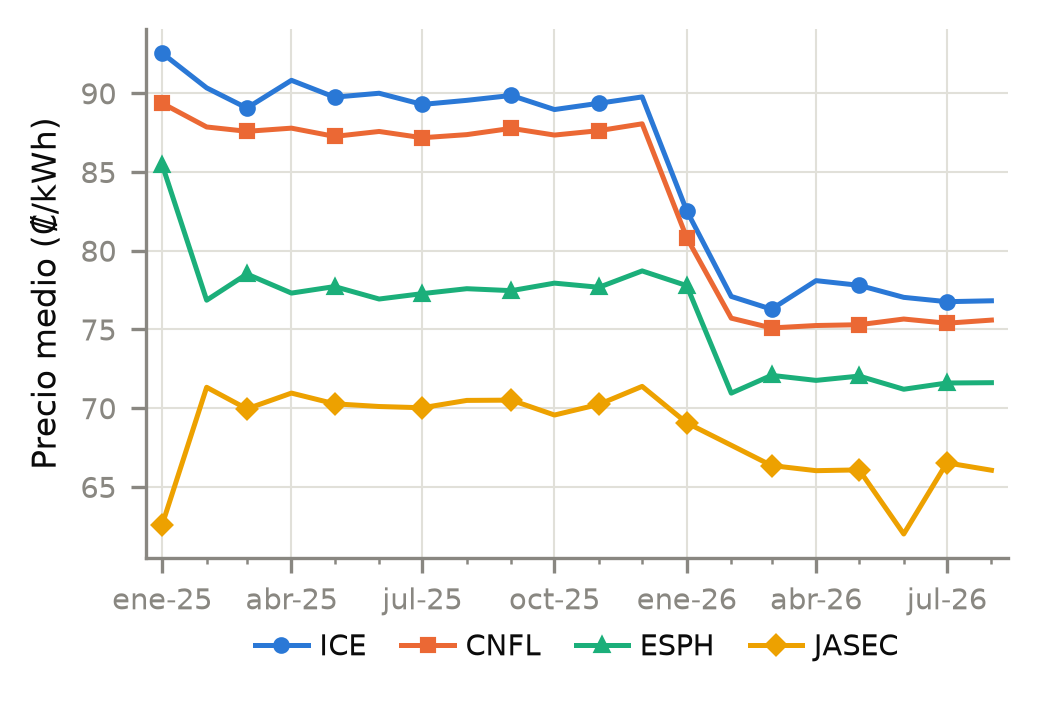
\includegraphics[width=\columnwidth,height=0.3\textheight,keepaspectratio]{figuras/01_precio_ponderado_mensual_operadores.png}
\vspace{-2mm}
\caption{Precio medio ponderado mensual por operador, enero de 2025 a agosto de 2026.}
\label{fig:precio-mensual}
\end{figure}
\FloatBarrier

El orden de los operadores se mantiene en los 20 meses del periodo: el ICE presenta siempre el precio ponderado m\'as alto, seguido de la CNFL, la ESPH y JASEC. Durante 2025 las cuatro series son estables, con variaciones mensuales cercanas a 1\,\crc/kWh. Entre diciembre de 2025 y febrero de 2026 se produce un descenso escalonado, coherente con el comportamiento de un precio fijado por resoluci\'on administrativa descrito en la Secci\'on~\ref{sec:aresep}: el ICE pasa de 89,77 a 77,09\,\crc/kWh ($-14{,}1$\,\%) y la CNFL de 88,06 a 75,71\,\crc/kWh ($-14{,}0$\,\%), ambos con la mayor ca\'ida en enero de 2026. La ESPH desciende un 9,9\,\%, principalmente en febrero, y JASEC solo un 5,2\,\%, de forma gradual. A partir de marzo de 2026 las series se estabilizan en un nuevo nivel, cercano a 77\,\crc/kWh para el ICE, 75\,\crc/kWh para la CNFL, 72\,\crc/kWh para la ESPH y 66\,\crc/kWh para JASEC. JASEC es adem\'as el operador m\'as estable del periodo, con una desviaci\'on est\'andar de 2,80\,\crc/kWh, frente a 6,27\,\crc/kWh del ICE.




% ---------------------------------
% ---------------------------------
\subsection{Comparaci\'on entre periodos equivalentes}

La Tabla~\ref{tab:trimestral} compara el I y el II trimestre de 2025 con los mismos trimestres de 2026 para cada operador, mediante el precio medio ponderado y la variaci\'on porcentual del precio, del ingreso y de las ventas. Julio y agosto de 2026 no participan de esta comparaci\'on, conforme a la delimitaci\'on del estudio (Secci\'on~\ref{sec:delimitacion}).

\begin{table}[htbp]
\caption{Comparaci\'on trimestral por operador, 2025 frente a 2026}
\label{tab:trimestral}
\centering
\scriptsize
\renewcommand{\arraystretch}{1.15}
\begin{tabular*}{\columnwidth}{@{\extracolsep{\fill}}llrrrrr@{}}
\hline
 & & \multicolumn{2}{c}{\textbf{Precio (\crc/kWh)}} & \multicolumn{3}{c}{\textbf{Variaci\'on (\%)}} \\
\textbf{Oper.} & \textbf{Trim.} & \textbf{2025} & \textbf{2026} & \textbf{Precio} & \textbf{Ingreso} & \textbf{Ventas} \\
\hline
ICE   & I  & 90,66 & 78,65 & $-$13,25 & $-$10,24 & $+$3,47 \\
ICE   & II & 90,20 & 77,65 & $-$13,91 & $-$7,51  & $+$7,44 \\
CNFL  & I  & 88,26 & 77,17 & $-$12,56 & $-$9,64  & $+$3,35 \\
CNFL  & II & 87,54 & 75,40 & $-$13,86 & $-$9,82  & $+$4,69 \\
ESPH  & I  & 80,30 & 73,60 & $-$8,35  & $-$8,24  & $+$0,12 \\
ESPH  & II & 77,31 & 71,66 & $-$7,31  & $-$7,30  & $+$0,01 \\
JASEC & I  & 67,96 & 67,67 & $-$0,43  & $+$6,00  & $+$6,47 \\
JASEC & II & 70,44 & 64,70 & $-$8,14  & $-$1,13  & $+$7,63 \\
\hline
\end{tabular*}
\end{table}
\FloatBarrier

En los cuatro operadores el precio ponderado del I y el II trimestre de 2026 es menor que el de 2025, aunque con magnitudes distintas. El ICE y la CNFL registran las mayores ca\'idas, entre el 12,6\,\% y el 13,9\,\%, y la ESPH presenta descensos de entre el 7,3\,\% y el 8,3\,\%, muy similares en ambos trimestres. Como las ventas no disminuyeron en ning\'un caso, la reducci\'on del ingreso en estos tres operadores responde al efecto precio y no a una contracci\'on del consumo; en la ESPH, cuyas ventas se mantuvieron pr\'acticamente constantes, el ingreso cae casi en la misma proporci\'on que el precio, mientras que en el ICE y la CNFL el crecimiento de las ventas, de entre el 3,3\,\% y el 7,4\,\%, aten\'ua parcialmente la ca\'ida del ingreso.

JASEC requiere una lectura particular. La ca\'ida casi nula de su precio en el I trimestre ($-$0,43\,\%) y el aumento del 6,00\,\% en su ingreso se explican principalmente por un precio at\'ipicamente bajo en enero de 2025 (62,58\,\crc/kWh, frente a cerca de 70\,\crc/kWh en el resto del a\~no), que reduce la base de comparaci\'on. Si se comparan \'unicamente febrero y marzo, el precio de JASEC desciende un 5,15\,\% y su ingreso crece apenas un 1,30\,\%. En el II trimestre, sin ese efecto, su precio cae un 8,14\,\%, una magnitud cercana a la de la ESPH, y su ingreso disminuye un 1,13\,\% pese al aumento de las ventas.

% ---------------------------------
\subsection{Efecto del Costo Variable de Generaci\'on (CVG)}

El efecto del CVG se calcul\'o, para cada operador y mes, como la diferencia entre el precio medio ponderado con CVG y sin CVG, ambos obtenidos con la Ecuaci\'on~\eqref{eq:precio_medio} sobre el agregado mensual. La Figura~\ref{fig:cvg} muestra el resultado.

\begin{figure}[!htb]
\centering
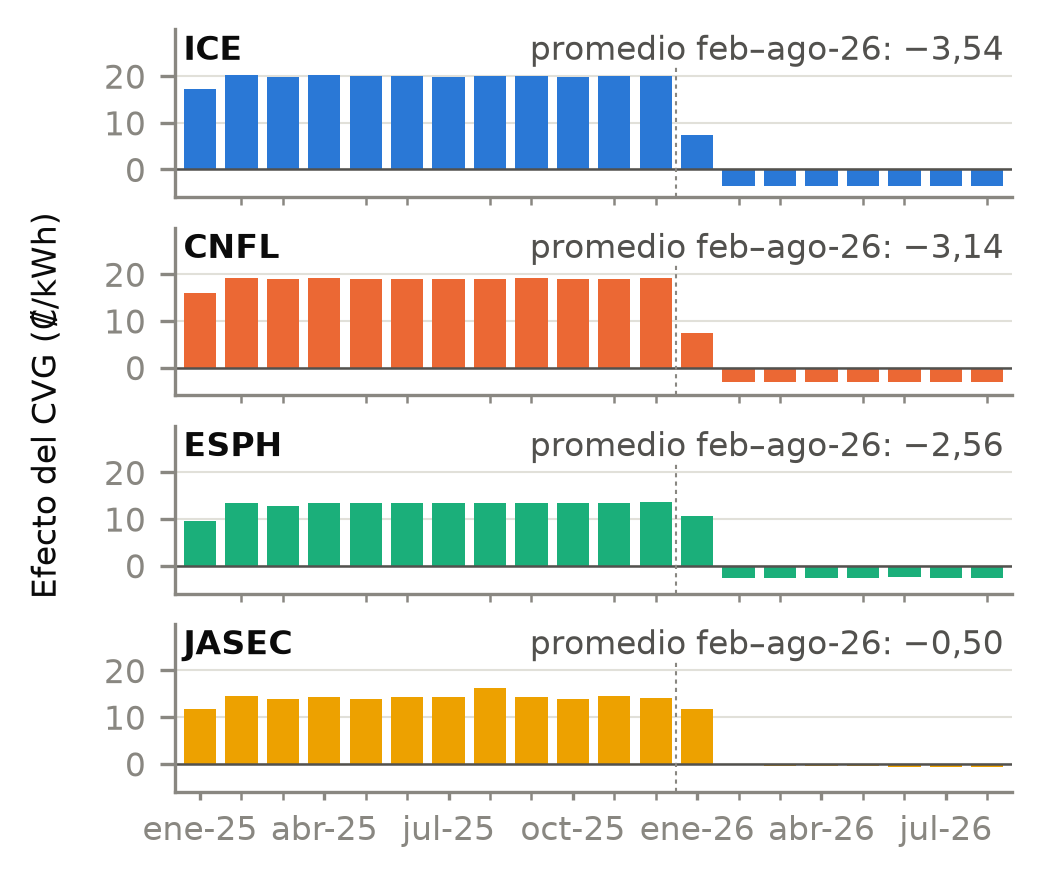
\includegraphics[width=\columnwidth]{figuras/03_efecto_cvg_operadores.png}
\caption{Efecto mensual del CVG sobre el precio medio ponderado por operador. Los valores positivos indican un recargo y los negativos un descuento.}
\label{fig:cvg}
\end{figure}
\FloatBarrier

Durante 2025 el CVG funcion\'o como un recargo estable: a\~nadi\'o en promedio entre 13,07\,\crc/kWh (ESPH) y 19,76\,\crc/kWh (ICE) al precio medio ponderado, con un m\'aximo mensual de 20,26\,\crc/kWh en el ICE en abril. En enero de 2026 el efecto todav\'ia fue positivo, aunque menor (entre 7,34 y 11,71\,\crc/kWh), y a partir de febrero de 2026 cambi\'o de signo en los cuatro operadores: entre febrero y agosto el CVG rest\'o en promedio entre 0,50\,\crc/kWh (JASEC) y 3,54\,\crc/kWh (ICE). Este cambio coincide con la ca\'ida del precio ponderado descrita en la secci\'on anterior y explica buena parte de ella. Es coherente adem\'as con la dependencia hidrol\'ogica del costo de generaci\'on se\~nalada en la Secci\'on~\ref{sec:electricidadCR}: el encarecimiento t\'ermico asociado a El Ni\~no de 2023--2024 se fue diluyendo, y hacia 2026 el ajuste extraordinario del CVG pas\'o de ser un recargo a un descuento.





% ---------------------------------
\section{Regresi\'on lineal de los precios medios}
\label{sec:regresion}

Para cuantificar la evoluci\'on del precio medio ponderado mensual (Secci\'on~\ref{sec:eda}) se ajustaron dos modelos de regresi\'on lineal por operador, con $t = 1, \dots, 20$ como \'indice del mes (enero de 2025 a agosto de 2026). Cada modelo se ajust\'o dos veces: con el precio ponderado que incluye el CVG (\texttt{ingresoConCVG}/\texttt{ventas}) y con el que lo excluye (\texttt{ingresoSinCVG}/\texttt{ventas}). La versi\'on sin CVG permite separar el comportamiento de la tarifa base del cambio de signo que el CVG experimenta a partir de febrero de 2026 (Figura~\ref{fig:cvg}).


% ---------------------------------
% ---------------------------------
\subsection{Regresi\'on lineal simple}

El primer modelo relaciona el precio con el tiempo mediante una sola recta por operador:
\begin{equation}
\text{precio}_t = \beta_0 + \beta_1\, t + \varepsilon_t,
\label{eq:reg_simple}
\end{equation}
donde $t = 1, \dots, 20$ es el \'indice del mes (enero de 2025 a agosto de 2026) y $\beta_1$ la variaci\'on mensual promedio del precio, en \crc/kWh por mes. La Tabla~\ref{tab:reg-simple} resume los coeficientes de ambas variantes del precio.

\begin{table}[htbp]
\caption{Regresi\'on lineal simple: pendiente mensual por operador}
\label{tab:reg-simple}
\centering
\scriptsize
\renewcommand{\arraystretch}{1.15}
\begin{tabular*}{\columnwidth}{@{\extracolsep{\fill}}llrcr@{}}
\hline
\textbf{Oper.} & \textbf{Precio} & \textbf{$\hat\beta_1$} & \textbf{IC 95\,\%} & \textbf{$R^2$} \\
\hline
ICE   & Con CVG & $-$0,941 & [$-$1,182; $-$0,700] & 0,79 \\
ICE   & Sin CVG & $+$0,681 & [$+$0,401; $+$0,961] & 0,59 \\
CNFL  & Con CVG & $-$0,880 & [$-$1,126; $-$0,635] & 0,76 \\
CNFL  & Sin CVG & $+$0,637 & [$+$0,390; $+$0,884] & 0,62 \\
ESPH  & Con CVG & $-$0,511 & [$-$0,691; $-$0,331] & 0,66 \\
ESPH  & Sin CVG & $+$0,528 & [$+$0,195; $+$0,862] & 0,38 \\
JASEC & Con CVG & $-$0,225 & [$-$0,431; $-$0,019] & 0,23 \\
JASEC & Sin CVG & $+$0,766 & [$+$0,515; $+$1,016] & 0,70 \\
\hline
\end{tabular*}
\end{table}

\textit{Precio con CVG.} La Figura~\ref{fig:reg-con} muestra las rectas ajustadas al precio con CVG.

\begin{figure}[!htb]
\centering
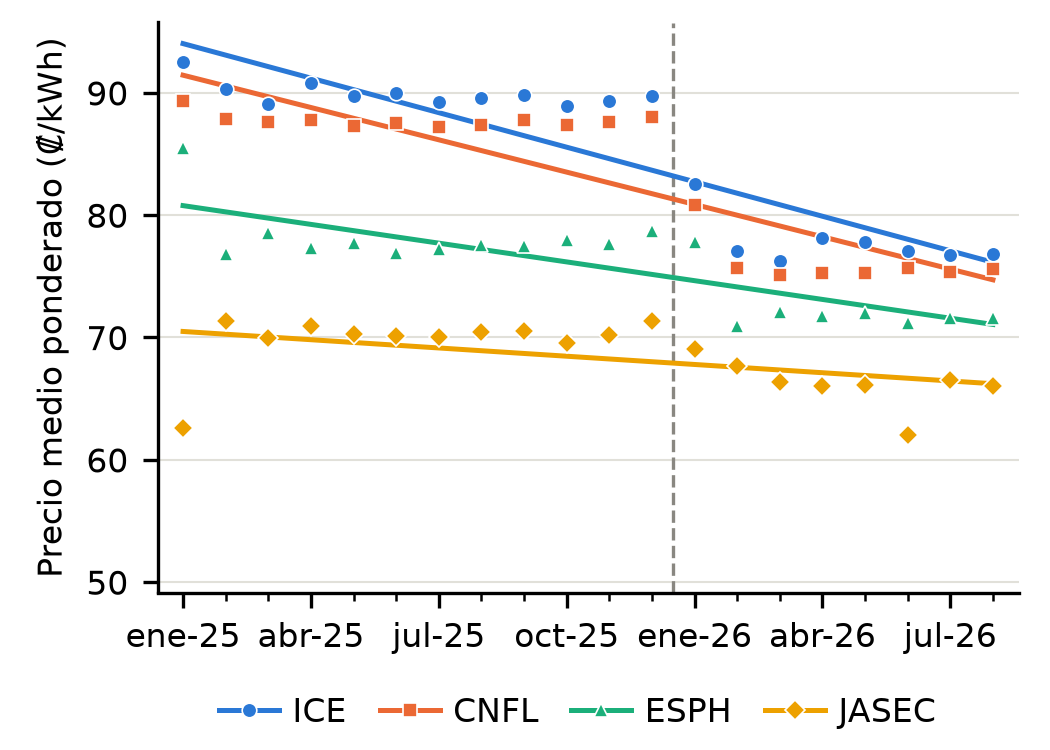
\includegraphics[width=\columnwidth]{figuras/07a_regresion_con_cvg.png}
\caption{Regresi\'on lineal simple del precio medio ponderado mensual con CVG. Los puntos son los precios mensuales, las l\'ineas las rectas ajustadas y la l\'inea discontinua separa 2025 de 2026.}
\label{fig:reg-con}
\end{figure}

La pendiente es negativa en los cuatro operadores: el ICE y la CNFL pierden cerca de 0,9\,\crc/kWh por mes, la ESPH 0,5\,\crc/kWh y JASEC 0,2\,\crc/kWh, este \'ultimo con un intervalo cercano al cero y un ajuste d\'ebil ($R^2 = 0{,}23$). Sin embargo, los puntos no descienden de forma gradual: el precio se mantiene en un nivel alto durante 2025, cae a inicios de 2026, con enero como mes de transici\'on, y desde febrero se estabiliza en un nivel menor. La recta reparte esa ca\'ida a lo largo de los 20 meses.

\textit{Precio sin CVG.} La Figura~\ref{fig:reg-sin} muestra el mismo ajuste para el precio sin CVG.

\begin{figure}[!htb]
\centering
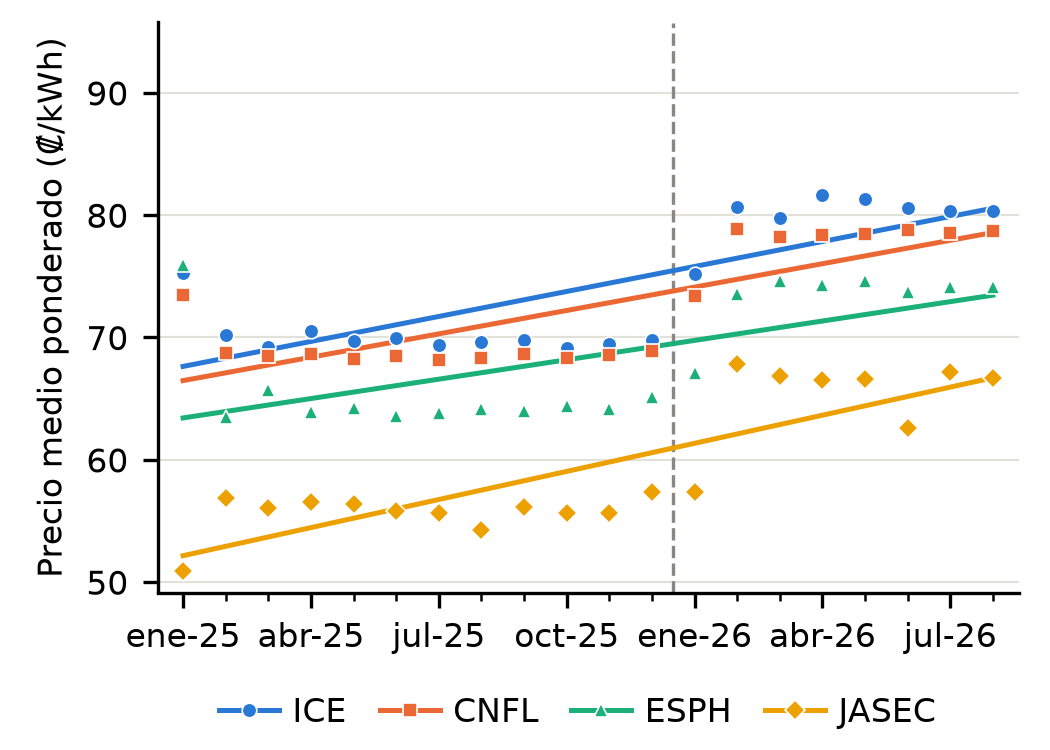
\includegraphics[width=\columnwidth]{figuras/07b_regresion_sin_cvg.png}
\caption{Regresi\'on lineal simple del precio medio ponderado mensual sin CVG, con la misma escala vertical que la Figura~\ref{fig:reg-con}.}
\label{fig:reg-sin}
\end{figure}
\FloatBarrier

En este caso el signo se invierte y la pendiente es positiva en los cuatro operadores, entre 0,53\,\crc/kWh por mes (ESPH) y 0,77\,\crc/kWh por mes (JASEC). El mejor ajuste es el de JASEC ($R^2 = 0{,}70$) y el m\'as d\'ebil el de la ESPH ($R^2 = 0{,}38$). Igual que con CVG, la serie no crece de forma continua: es estable en 2025, sube a inicios de 2026 y vuelve a estabilizarse desde febrero.

\textit{Contraste entre ambas variantes.} Las pendientes de signo opuesto responden al mismo hecho: en 2026 la tarifa base aumenta, mientras el CVG pasa de recargo a rebaja, de modo que el precio que paga el usuario baja aunque el precio sin CVG suba. En ambas variantes la recta resume un escal\'on y no una tendencia, lo que confirma el estad\'istico de Durbin-Watson, que va de 0,45 a 1,38, muy por debajo de 2, y revela autocorrelaci\'on fuerte en los residuos. Por ello los valores $p$ de este modelo no se interpretan, lo que motiva el modelo con indicador de la subsecci\'on siguiente.















% ---------------------------------
\subsection{Regresi\'on con indicador de 2026}

Para separar el cambio de nivel de la tendencia, el segundo modelo a\~nade una variable indicadora:
\begin{equation}
\text{precio}_t = \beta_0 + \beta_1\, t + \beta_2\, D_{2026,t} + \varepsilon_t,
\label{eq:reg_indicador}
\end{equation}
donde $D_{2026,t}$ vale 1 desde febrero de 2026 ($t \geq 14$), primer mes en que el CVG resta al precio, y 0 antes. Enero de 2026 ($t = 13$) se excluy\'o del ajuste por ser un mes de transici\'on, en el que el CVG se redujo sin llegar a\'un a ser negativo, por lo que cada serie cuenta con $n = 19$ observaciones. As\'i, $\beta_2$ mide el cambio de nivel del precio (\crc/kWh) y $\beta_1$ la tendencia mensual dentro de cada periodo. Los errores est\'andar se calcularon con la correcci\'on de Newey-West (rezago 2) y los valores $p$ con la distribuci\'on $t$ de $n-3$ grados de libertad. La Tabla~\ref{tab:reg-indicador} resume los coeficientes de ambas variantes del precio.

\begin{table}[htbp]
\caption{Regresi\'on con indicador de 2026: coeficientes por operador}
\label{tab:reg-indicador}
\centering
\scriptsize
\renewcommand{\arraystretch}{1.15}
\begin{tabular*}{\columnwidth}{@{\extracolsep{\fill}}llrrrr@{}}
\hline
\textbf{Oper.} & \textbf{Precio} & \textbf{$\hat\beta_1$} & \textbf{$\hat\beta_2$} & \textbf{$R^2$} & \textbf{DW} \\
\hline
ICE   & Con CVG & $-$0,141* & $-$11,34* & 0,99 & 1,90 \\
ICE   & Sin CVG & $-$0,218  & $+$12,78* & 0,95 & 1,46 \\
CNFL  & Con CVG & $-$0,050  & $-$11,78* & 0,99 & 1,21 \\
CNFL  & Sin CVG & $-$0,153  & $+$11,24* & 0,96 & 1,23 \\
ESPH  & Con CVG & $-$0,203  & $-$4,55*  & 0,79 & 1,66 \\
ESPH  & Sin CVG & $-$0,353  & $+$12,65* & 0,77 & 1,59 \\
JASEC & Con CVG & $+$0,192  & $-$5,99*  & 0,51 & 1,70 \\
JASEC & Sin CVG & $+$0,102  & $+$9,64*  & 0,92 & 1,79 \\
\hline
\multicolumn{6}{@{}l@{}}{\footnotesize $\hat\beta_1$ en \crc/kWh por mes; $\hat\beta_2$ en \crc/kWh. * Significativo al 5\,\% (Newey-West).} \\
\end{tabular*}
\end{table}

\subsubsection{Precio con CVG}

\begin{figure}[!htb]
\centering
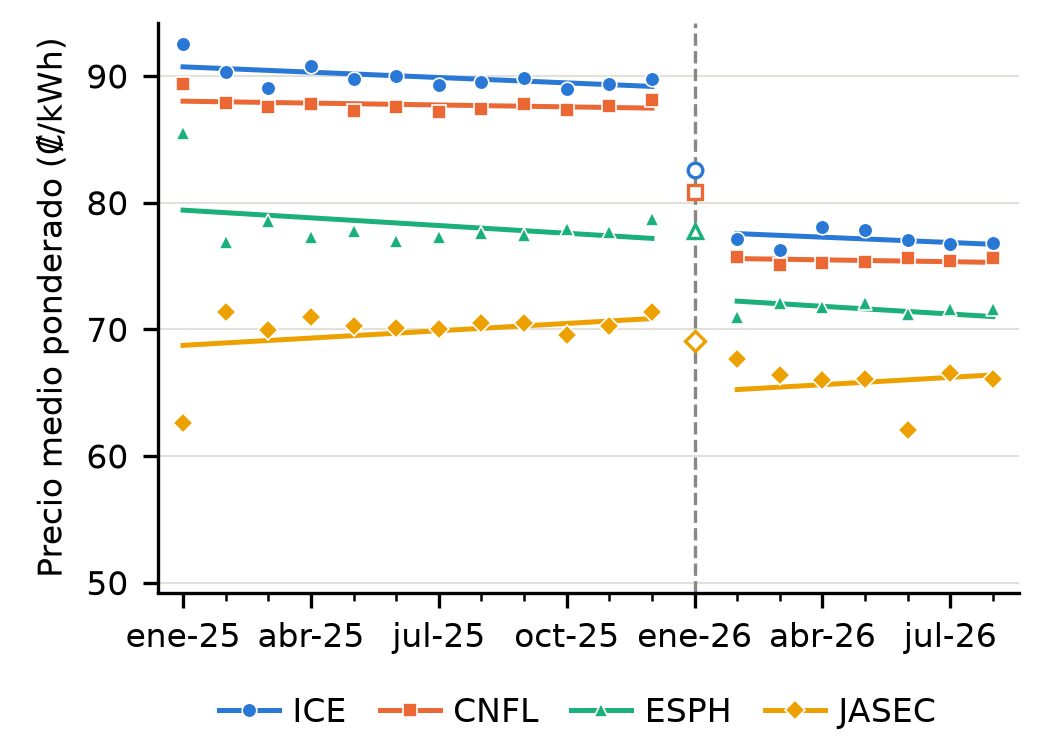
\includegraphics[width=\columnwidth]{figuras/10a_indicador_con_cvg.png}
\caption{Regresi\'on con indicador de 2026 del precio medio ponderado mensual con CVG. Las l\'ineas son los tramos ajustados antes y despu\'es del cambio de nivel; el marcador hueco corresponde a enero de 2026, excluido del ajuste.}
\label{fig:ind-con}
\end{figure}

Con CVG (Figura~\ref{fig:ind-con}), el cambio de nivel es negativo y significativo en los cuatro operadores: el precio cae 11,3\,\crc/kWh en el ICE y 11,8\,\crc/kWh en la CNFL, y bastante menos en JASEC (6,0\,\crc/kWh) y la ESPH (4,6\,\crc/kWh). Fuera del escal\'on la tendencia es casi nula: solo la pendiente del ICE ($-$0,14\,\crc/kWh por mes) resulta significativa, y en el l\'imite del umbral. El ajuste es muy alto en el ICE y la CNFL ($R^2 = 0{,}99$), alto en la ESPH (0,79) y moderado en JASEC (0,51), cuya serie incluye el valor at\'ipicamente bajo de enero de 2025.

\subsubsection{Precio sin CVG}

\begin{figure}[!htb]
\centering
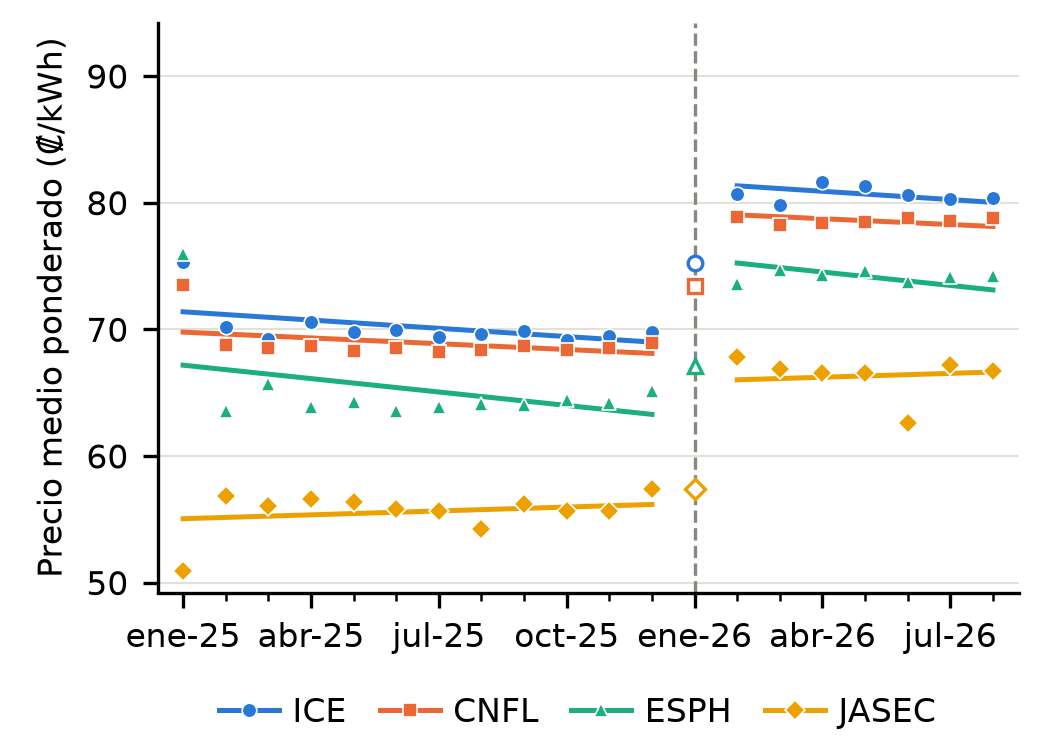
\includegraphics[width=\columnwidth]{figuras/10b_indicador_sin_cvg.png}
\caption{Regresi\'on con indicador de 2026 del precio medio ponderado mensual sin CVG, con la misma escala vertical que la Figura~\ref{fig:ind-con}.}
\label{fig:ind-sin}
\end{figure}

Sin CVG (Figura~\ref{fig:ind-sin}) el escal\'on cambia de signo: el precio base sube de forma significativa en los cuatro operadores, entre 9,6\,\crc/kWh (JASEC) y 12,8\,\crc/kWh (ICE), con 11,2\,\crc/kWh en la CNFL y 12,6\,\crc/kWh en la ESPH. Ninguna pendiente es significativa y todas son menores que 0,4\,\crc/kWh por mes en valor absoluto, de modo que, descontado el escal\'on, el precio base se mantiene estable dentro de cada periodo. El $R^2$ va de 0,77 (ESPH) a 0,96 (CNFL).

\subsubsection{Contraste entre ambas variantes}

Como el modelo es lineal, la diferencia entre los dos escalones equivale al cambio de nivel estimado del propio CVG: 24,1\,\crc/kWh en el ICE, 23,0\,\crc/kWh en la CNFL, 17,2\,\crc/kWh en la ESPH y 15,6\,\crc/kWh en JASEC. En febrero de 2026 el precio base subi\'o, pero el CVG pas\'o de sumar a restar en una magnitud mayor, por lo que el precio final baj\'o. Esto explica tambi\'en las diferencias entre operadores: en el ICE y la CNFL el giro del CVG es cerca del doble del aumento de la tarifa base y el precio cae unos 11\,\crc/kWh, mientras que en la ESPH y JASEC el giro es menor en proporci\'on y la ca\'ida se reduce a entre 4,6 y 6,0\,\crc/kWh.

% ---------------------------------
\subsection{Contraste entre ambos modelos}

La regresi\'on simple sugiere tendencias opuestas, negativa con CVG y positiva sin CVG, pero su Durbin-Watson (0,45 a 1,38) indica que una recta \'unica no describe bien las series. Al incorporar el indicador, el $R^2$ con CVG pasa de un rango de 0,23--0,79 a uno de 0,51--0,99, y sin CVG de 0,38--0,70 a 0,77--0,96; el Durbin-Watson sube a valores entre 1,21 y 1,90, m\'as cercanos a 2, y las pendientes pr\'acticamente desaparecen. Ambos modelos coinciden en el diagn\'ostico, pero el segundo lo precisa: los precios medios de los operadores no siguen una tendencia, sino que se comportan como un nivel que cambia una vez, entre enero y febrero de 2026, y luego se mantiene estable, lo que confirma desde el modelado lo observado en la Secci\'on~\ref{sec:eda}.

\textbf{Limitaciones.} Con 19 observaciones por serie, los intervalos de confianza son amplios y la significancia de las pendientes es sensible al m\'etodo de c\'alculo de los errores, como ocurre con la del ICE. Los resultados describen el periodo observado y no deben extrapolarse como pron\'ostico de los meses siguientes, en particular porque el precio depende de resoluciones tarifarias futuras.


% ---------------------------------
\subsection{Evaluaci\'on predictiva y escenario a diciembre de 2026}
\label{sec:pronostico}

Para evaluar la capacidad predictiva de los modelos, cada serie se dividi\'o en un periodo de entrenamiento, de enero de 2025 a abril de 2026 ($t = 1, \dots, 16$), y uno de prueba, de mayo a agosto de 2026 ($t = 17, \dots, 20$). Desde abril de 2026 se pronosticaron los cuatro meses siguientes con tres modelos: un pron\'ostico ingenuo, que repite el \'ultimo valor observado; la regresi\'on con indicador de la Ecuaci\'on~\eqref{eq:reg_indicador}; y un modelo ARIMAX$(p,0,q)$, con $p, q \in \{0,1\}$, que incorpora como regresores el escal\'on $D_{2026,t}$ y un pulso para enero de 2026, y cuyo orden se eligi\'o por el criterio de informaci\'on de Akaike (AIC). No se incluy\'o un componente estacional, ya que un modelo SARIMA con periodo de 12 meses requiere varios ciclos anuales completos~\cite{r13}. El error se midi\'o con el MAE, el RMSE y el MAPE (Tabla~\ref{tab:pronostico}).

\begin{table}[htbp]
\caption{Error del pron\'ostico de mayo a agosto de 2026, promedio de los cuatro operadores}
\label{tab:pronostico}
\centering
\scriptsize
\renewcommand{\arraystretch}{1.15}
\begin{tabular*}{\columnwidth}{@{\extracolsep{\fill}}llrrr@{}}
\hline
\textbf{Modelo} & \textbf{Precio} & \textbf{MAE} & \textbf{RMSE} & \textbf{MAPE (\%)} \\
\hline
Ingenuo            & Con CVG & 0,67 & 0,93 & 0,96 \\
                   & Sin CVG & 0,68 & 0,92 & 0,96 \\
Reg. con indicador & Con CVG & 1,04 & 1,23 & 1,54 \\
                   & Sin CVG & 1,23 & 1,44 & 1,72 \\
ARIMAX             & Con CVG & 0,93 & 1,10 & 1,36 \\
                   & Sin CVG & 1,08 & 1,33 & 1,50 \\
\hline
\multicolumn{5}{@{}l@{}}{\footnotesize MAE y RMSE en \crc/kWh.} \\
\end{tabular*}
\end{table}

El pron\'ostico ingenuo obtuvo el menor error promedio en ambas variantes del precio: con CVG, su MAE fue de 0,67\,\crc/kWh, frente a 0,93 del ARIMAX y 1,04 de la regresi\'on con indicador. En el ICE, la CNFL y la ESPH, el AIC seleccion\'o un ARIMAX sin componentes autorregresivos ni de media m\'ovil, equivalente a la regresi\'on con indicador; solo en JASEC eligi\'o un componente autorregresivo de orden 1, lo que explica la peque\~na ventaja promedio del ARIMAX. Los tres modelos se equivocan en promedio menos de un 2\,\%, y aunque en el ICE la regresi\'on y el ARIMAX superan al ingenuo, en promedio ninguno lo hace: con precios casi constantes desde febrero de 2026, el mejor pron\'ostico de corto plazo es el \'ultimo valor observado. El resultado es coherente con un precio que cambia por resoluciones administrativas y no por la din\'amica propia de la serie.

Con el mismo procedimiento, el ARIMAX se reajust\'o con los 20 meses y se pronostic\'o el precio de setiembre a diciembre de 2026 (Figura~\ref{fig:pronostico} y Tabla~\ref{tab:escenario}). Se trata de un escenario sin nuevas resoluciones tarifarias, que supone que el nivel vigente desde febrero de 2026 se mantiene. En los cuatro operadores, el precio con CVG de diciembre queda a menos de 1\,\crc/kWh de su valor de agosto. Los intervalos de predicci\'on del 95\,\% son estrechos en el ICE y la CNFL (entre $\pm$0,8 y $\pm$1,3\,\crc/kWh) y m\'as amplios en la ESPH y JASEC (cerca de $\pm$4\,\crc/kWh), cuyas series son m\'as irregulares. Estos intervalos subestiman la incertidumbre real, ya que no incluyen el error de estimaci\'on de los coeficientes ni posibles ajustes tarifarios, como el del CVG para 2027.

\begin{figure}[!htb]
\centering
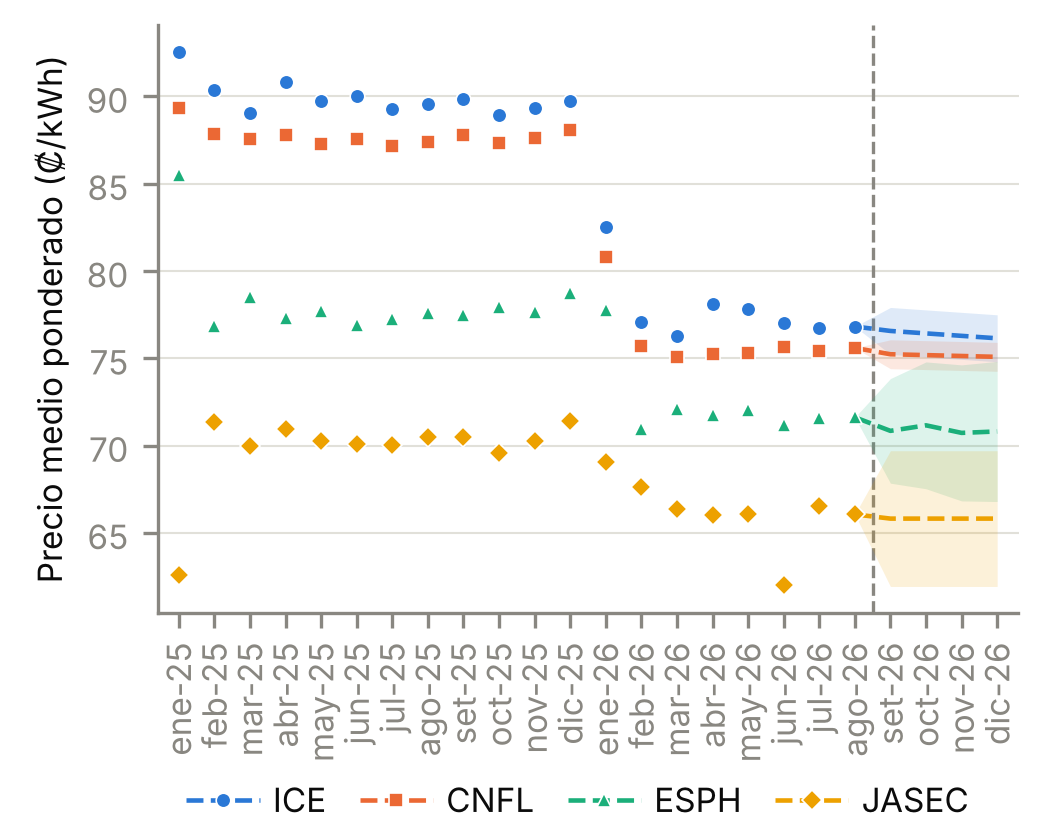
\includegraphics[width=\columnwidth]{figuras/13_pronostico_con_cvg.png}
\caption{Precio medio ponderado mensual con CVG observado (enero de 2025 a agosto de 2026) y escenario ARIMAX de setiembre a diciembre de 2026, con su intervalo de predicci\'on del 95\,\%.}
\label{fig:pronostico}
\end{figure}

\begin{table}[htbp]
\caption{Escenario del precio con CVG a diciembre de 2026 (\crc/kWh)}
\label{tab:escenario}
\centering
\scriptsize
\renewcommand{\arraystretch}{1.15}
\begin{tabular*}{\columnwidth}{@{\extracolsep{\fill}}lcrrc@{}}
\hline
\textbf{Oper.} & \textbf{Orden} & \textbf{Ago. 2026} & \textbf{Dic. 2026} & \textbf{IC 95\,\%} \\
\hline
ICE   & (0,0,0) & 76,82 & 76,14 & [74,80; 77,49] \\
CNFL  & (0,0,0) & 75,59 & 75,08 & [74,25; 75,91] \\
ESPH  & (1,0,0) & 71,62 & 70,81 & [66,79; 74,82] \\
JASEC & (0,0,0) & 66,06 & 65,81 & [61,92; 69,70] \\
\hline
\multicolumn{5}{@{}l@{}}{\footnotesize Ago. 2026: valor observado. Dic. 2026: pron\'ostico ARIMAX.} \\
\end{tabular*}
\end{table}
\FloatBarrier

\textbf{Limitaciones.} La evaluaci\'on predictiva se basa en solo cuatro meses de prueba y en tres meses de entrenamiento posteriores al cambio de nivel, por lo que las diferencias entre modelos son orientativas. El escenario a diciembre de 2026 es v\'alido solo a corto plazo y bajo el supuesto de que no haya nuevas resoluciones tarifarias.


% ---------------------------------
\section{Discusi\'on}
\label{sec:discusion}

Los resultados muestran que la reducci\'on del precio medio de la electricidad en 2026 no responde a una baja de las tarifas base, sino al cambio de signo del CVG. Sin este componente, el precio de los cuatro operadores aument\'o entre 9,6 y 12,8\,\crc/kWh; con \'el, disminuy\'o entre 4,6 y 11,8\,\crc/kWh, porque el CVG pas\'o de a\~nadir en promedio entre 13,07 y 19,76\,\crc/kWh en 2025 a restar entre 0,50 y 3,54\,\crc/kWh desde febrero de 2026. Para el usuario, el resultado neto fue un precio menor, aunque el precio sin CVG se encareci\'o.

Este comportamiento es coherente con la naturaleza regulada del precio descrita en la Secci\'on~\ref{sec:aresep}. Las series no evolucionan de forma gradual, sino que se mantienen estables durante meses y cambian de nivel en fechas concretas, en este caso entre enero y febrero de 2026. Por ello la regresi\'on simple, que supone una tendencia continua, produjo pendientes de signo opuesto y residuos con fuerte autocorrelaci\'on, mientras que el modelo con indicador explic\'o entre el 51 y el 99\,\% de la variabilidad con pendientes casi nulas. En un sistema regulado conviene, entonces, modelar el precio como una sucesi\'on de niveles asociados a decisiones tarifarias y no como una tendencia, lo que distingue este caso de los mercados mayoristas liberalizados que predominan en la literatura~\cite{r12}.

La magnitud del efecto difiri\'o entre operadores. En el ICE y la CNFL el giro del CVG, de 23 a 24\,\crc/kWh, fue cerca del doble del aumento del precio base y produjo las mayores ca\'idas, tanto en el modelo como en la comparaci\'on trimestral (entre 12,6 y 13,9\,\%). En la ESPH y JASEC el giro fue menor, de 15,6 a 17,2\,\crc/kWh, y la ca\'ida tambi\'en. Los operadores tampoco cambiaron al mismo tiempo: el ICE y la CNFL registraron la mayor parte de su baja en enero de 2026, mientras que la ESPH la concentr\'o en febrero.

En cuanto a los ingresos, las ventas no disminuyeron en ning\'un operador, por lo que la ca\'ida del ingreso con CVG en 2026 se explica por el precio y no por el consumo. En el ICE y la CNFL el crecimiento de las ventas amortigu\'o esa ca\'ida, mientras que en la ESPH, con ventas estables, el ingreso baj\'o casi en la misma proporci\'on que el precio. Debe considerarse, sin embargo, que el CVG traslada un costo de generaci\'on, por lo que una menor recaudaci\'on por este concepto no implica necesariamente un menor margen para las distribuidoras; este aspecto no puede evaluarse con los datos utilizados. 

La evaluaci\'on predictiva refuerza esta interpretaci\'on. Como los precios se mantienen casi constantes desde febrero de 2026, el pron\'ostico ingenuo result\'o en promedio m\'as preciso que la regresi\'on con indicador y que el ARIMAX, y el escenario a diciembre de 2026 anticipa precios muy cercanos a los de agosto. En un precio regulado, la principal fuente de cambio son las resoluciones tarifarias y el ajuste del CVG, que ning\'un modelo basado solo en la serie hist\'orica puede anticipar; por ello estos pron\'osticos son \'utiles solo a corto plazo y bajo el supuesto expl\'icito de que no haya nuevas resoluciones.

El estudio tiene limitaciones que acotan el alcance de estas conclusiones. Con 20 meses de datos no es posible estimar la estacionalidad anual ni ajustar con confiabilidad los modelos de pron\'ostico descritos en el marco te\'orico, como SARIMAX o Prophet, que requieren varios ciclos anuales~\cite{r13}. Adem\'as, el an\'alisis no incorpora las fechas de las resoluciones tarifarias, por lo que el cambio de nivel se ubic\'o a partir de los datos y no de los actos administrativos que lo originaron, ni separa el efecto precio del efecto composici\'on.

% ---------------------------------
\section{Conclusiones}
\label{sec:conclusiones}

A partir de los datos abiertos de la ARESEP y de un flujo reproducible en Python, este trabajo describi\'o y model\'o el precio medio de la electricidad de los cuatro principales operadores de distribuci\'on de Costa Rica entre enero de 2025 y agosto de 2026. Las principales conclusiones son las siguientes:
\begin{itemize}
\item La jerarqu\'ia de precios entre operadores es estable: el ICE tuvo el precio ponderado m\'as alto en los 20 meses, seguido de la CNFL, la ESPH y JASEC.
\item En el I y el II trimestre de 2026 el precio ponderado fue menor que en los mismos trimestres de 2025 en los cuatro operadores, con ca\'idas de hasta 13,9\,\%, sin que disminuyeran las ventas, por lo que la reducci\'on del ingreso responde al efecto precio.
\item El CVG pas\'o de ser un recargo en 2025 a un descuento desde febrero de 2026, y ese cambio explica la baja del precio final: sin CVG, el precio de los cuatro operadores aument\'o entre 9,6 y 12,8\,\crc/kWh.
\item Los precios regulados se comportan como niveles que cambian en fechas puntuales y no como tendencias. El modelo con variable indicadora describe mejor las series que la recta simple, con $R^2$ de hasta 0,99 y un Durbin-Watson m\'as cercano a 2, por lo que es el enfoque recomendable para este tipo de datos.

\item En la evaluaci\'on fuera de muestra de mayo a agosto de 2026, ni la regresi\'on con indicador ni el modelo ARIMAX superaron en promedio al pron\'ostico ingenuo, con errores porcentuales menores al 2\,\%. El escenario a diciembre de 2026, sin nuevas resoluciones, mantiene el precio con CVG a menos de 1\,\crc/kWh de su nivel de agosto.

\end{itemize}

Como trabajo futuro se propone incorporar las fechas de las resoluciones tarifarias de la ARESEP como variables del modelo, extender la serie a m\'as a\~nos para aplicar modelos de pron\'ostico con estacionalidad, como SARIMAX o Prophet, separar el efecto precio del efecto composici\'on por tipo de tarifa y analizar las cooperativas con la misma metodolog\'ia, como un grupo independiente.



% ---------------------------------
% REFERENCIAS
% ---------------------------------
\begin{thebibliography}{00}

\bibitem{r1} Autoridad Reguladora de los Servicios P\'ublicos, ``Electricidad,'' San Jos\'e, Costa Rica. [En l\'inea]. Disponible: \url{https://aresep.go.cr/electricidad/}

\bibitem{r2} Grupo ICE, ``Datos abiertos: estad\'isticas del sector el\'ectrico,'' San Jos\'e, Costa Rica. [En l\'inea]. Disponible: \url{https://www.grupoice.com/wps/portal/ICE/Transparencia/datos-abiertos/da-estadisticas}

\bibitem{r3} Asamblea Legislativa de la Rep\'ublica de Costa Rica, \emph{Ley N.\textsuperscript{o} 7593, Ley de la Autoridad Reguladora de los Servicios P\'ublicos}, San Jos\'e, Costa Rica, 1996. [En l\'inea]. Disponible: \url{https://www.sutel.go.cr/sites/default/files/normativas/ley_de_la_autoridad_reguladora_de_los_servicios_publicos_aresep_ley_7593.pdf}

\bibitem{r4} Autoridad Reguladora de los Servicios P\'ublicos, ``Metodolog\'ias de electricidad,'' San Jos\'e, Costa Rica. [En l\'inea]. Disponible: \url{https://aresep.go.cr/electricidad/metodologias/}

\bibitem{r5} Autoridad Reguladora de los Servicios P\'ublicos, ``Tarifas vigentes de electricidad,'' San Jos\'e, Costa Rica. [En l\'inea]. Disponible: \url{https://aresep.go.cr/electricidad/tarifas/}

\bibitem{r6} Autoridad Reguladora de los Servicios P\'ublicos, ``Precios medios'' [conjunto de datos abiertos], San Jos\'e, Costa Rica. [En l\'inea]. Disponible: \url{https://aresep.go.cr/datos-abiertos/precios-medios/}

\bibitem{r7} T. Hong and S. Fan, ``Probabilistic electric load forecasting: A tutorial review,'' \emph{International Journal of Forecasting}, vol. 32, no. 3, pp. 914--938, 2016, doi: 10.1016/j.ijforecast.2015.11.011.

\bibitem{r8} L. Wang, Y. Sun and Q. Wang, ``China's Electricity Pricing System for Promoting Common Wealth: Mechanism Path and Analysis,'' in \emph{2024 5th Int. Conf. Clean Energy and Electric Power Engineering (ICCEPE)}, Yangzhou, China, 2024, pp. 1409--1412, doi: 10.1109/ICCEPE62686.2024.10931482.

\bibitem{r9} ``Modernizaci\'on de las tarifas el\'ectricas en Costa Rica -- hacia la senda de la eficiencia,'' \emph{Pol\'itica Econ\'omica y Desarrollo Sostenible}, vol. 8, n.\textsuperscript{o} 2, pp. 1--17, 2023, doi: 10.15359/peds.8-2.2.

\bibitem{r10} J. W. Tukey, \emph{Exploratory Data Analysis}. Reading, MA, USA: Addison-Wesley, 1977.

\bibitem{r11} D. M. Blei and P. Smyth, ``Science and data science,'' \emph{Proceedings of the National Academy of Sciences}, vol. 114, no. 33, pp. 8689--8692, 2017.

\bibitem{r12} R. Weron, ``Electricity price forecasting: A review of the state-of-the-art with a look into the future,'' \emph{International Journal of Forecasting}, vol. 30, no. 4, pp. 1030--1081, 2014, doi: 10.1016/j.ijforecast.2014.08.008.

\bibitem{r13} G. E. P. Box, G. M. Jenkins, G. C. Reinsel and G. M. Ljung, \emph{Time Series Analysis: Forecasting and Control}, 5th ed. Hoboken, NJ, USA: Wiley, 2015.

\bibitem{r14} S. J. Taylor and B. Letham, ``Forecasting at scale,'' \emph{The American Statistician}, vol. 72, no. 1, pp. 37--45, 2018, doi: 10.1080/00031305.2017.1380080.

\bibitem{r15} L. Breiman, ``Random forests,'' \emph{Machine Learning}, vol. 45, no. 1, pp. 5--32, 2001, doi: 10.1023/A:1010933404324.

\bibitem{r16} T. Chen and C. Guestrin, ``XGBoost: A scalable tree boosting system,'' in \emph{Proc. 22nd ACM SIGKDD Int. Conf. Knowledge Discovery and Data Mining}, San Francisco, CA, USA, 2016, pp. 785--794, doi: 10.1145/2939672.2939785.

\bibitem{r17} A. Nagpal and G. Gabrani, ``Python for Data Analytics, Scientific and Technical Applications,'' in \emph{2019 Amity Int. Conf. Artificial Intelligence (AICAI)}, Dubai, United Arab Emirates, 2019, pp. 140--145, doi: 10.1109/AICAI.2019.8701341.

\bibitem{r18} J. G. Rodriguez Rivas y S. Rodr\'iguez Castillo, ``Uso de Python para el an\'alisis de datos aplicado en la investigaci\'on,'' \emph{INCAING}, vol. 5, n.\textsuperscript{o} 34, pp. 33--40, nov. 2022. [En l\'inea]. Disponible: \url{https://ojsincaing.com.mx/index.php/ediciones/article/view/188}

\end{thebibliography}

\end{document}